\documentclass[a4 paper]{article}
%\usepackage{minted}           %embedding code
\usepackage{amsmath, amsthm, amsfonts} %always use amsmath for symbols, amsthm for theorems 
\usepackage{graphicx}  % for pictures
%\usepackage{lipsum}  % for test text
\usepackage{multicol}    % for multicollumn text
\usepackage[bottom=2.5cm]{geometry}   %to set the margins to your liking
\usepackage[skip = 10pt, indent = 30pt]{parskip}      %to set the distance between paragraphs
\usepackage{tcolorbox}           %for literal color boxes
%\usepackage{witharrows}             % understandable, arrows for equations
\usepackage{tikz}                   %drawings and diagrams
\usetikzlibrary{positioning}        %tikz library for positioning (of nodes?)
\usepackage{pgfplots}               %plotting and graphs
\pgfplotsset{compat=1.18, width = 10cm}
\usepackage{hyperref}
\hypersetup{colorlinks = true, linkcolor = black, urlcolor = blue}
%\usepackage{fancyvrb}           % fancy formatting of verbatim
%\usepackage{fancyhdr, lastpage}
%\pagestyle{fancy} 
%\lhead{Relat\'orio experimento 4}
%\rhead{FisExpI}
%\cfoot{Página \thepage \ de \pageref{LastPage}}
%\usepackage[Bjornstrup]{fncychap} %Sonny, Glenn, Lenny, Conny, Rejne, Bjarne, Bjornstrup
%\usepackage{xcolor}      %color text
%\usepackage{siunitx}    %for SI units
\usepackage{setspace}
\onehalfspacing
\usepackage{cleveref}
\usepackage[brazil]{babel}
\usepackage{caption}
\usepackage{subcaption}
\usepackage{pdfpages}
\usepackage{booktabs}
\usepackage{multirow}
\usepackage{textcomp}
\usepackage{amssymb}
\usepackage[document]{ragged2e}
\usepackage{bm}
\usepackage{empheq}




%\setlength{\hoffset}{-2cm}
%\setlength{\voffset}{1.5cm}                     %control your margins however you want!
%\setlength{\marginparwidth}{2cm}
%\setlength{\oddsidemargin}{0cm}

%\newtheorem{theorem}{Theorem}[section]               %how you call it and how you display it
%\newtheorem{corollary}{Corollary}[theorem]


\newcommand{\parag}{\hspace{30pt}}
%\newcommand{\pd}[2]{\frac{\partial#1}{\partial#2}}


\begin{document}


\justifying
\begin{center}{\large Laboratório de Circuitos Elétricos - 02/2024 - Turma 05}\\
{\large \textbf{Experimento 7}}\\ 
09/01/2025
\end{center}

\vspace{500pt}
 \noindent\textbf{Grupo 5:}\\
 Yuri Shumyatsky - 231012826\\
Vinicius de Melo Moraes - 231036274\\



\vspace{30pt}
\newpage

\section{Introdução}
\parag O experimento tem como objetivo principal analisar as respostas em frequência de circuitos que apresentam resistência, indutância e capacitância em diferentes configurações. Por meio da variação da frequência do sinal de entrada, são obtidos os comportamentos de amplitude e fase, que são representados graficamente no Diagrama de Bode. Este tipo de análise permite identificar características importantes do circuito, como frequência de ressonância, largura de banda e comportamento em altas e baixas frequências. A abordagem experimental possibilita compreender a influência dos parâmetros do circuito sobre a resposta em frequência e sua aplicação em filtros e sistemas de controle.

\section{Materiais}
	\begin{itemize}
	\item National Instruments Elvis II
	\item 1 capacitor de 100n$F$
	\item 1 resistor de 47$\Omega$
	\item 1 indutor de 1mH
	\end{itemize}

\newpage
\section{Procedimentos}
\parag Como já é de costume, são feitas as medidas dos valores de todos os componentes do ciruito e esses valores são comparados com os nominais. O resultado é o disposto na Tabela 1.

\vspace{5pt}
\begin{table}[h]
\centering
\begin{tabular}{|c|c|c|c|}
\hline
\textbf{Grandeza} & \textbf{Valor nominal} & \textbf{Valor medido} & \textbf{Erro (\%) }\\\hline
R & 47$\Omega$ & 47.359$\Omega$ & 0.76 \\\hline 
L & 1mH & 0.863mH & 13.70 \\\hline 
C & 100nF & 107.500nF & 7.50 \\\hline 
\end{tabular}
\caption*{Tabela 1: Valores dos componentes}
\end{table}

Em seguida, esses componentes são dispostos na configuração mostrada na Figura 1.

\begin{table}[h]
\centering
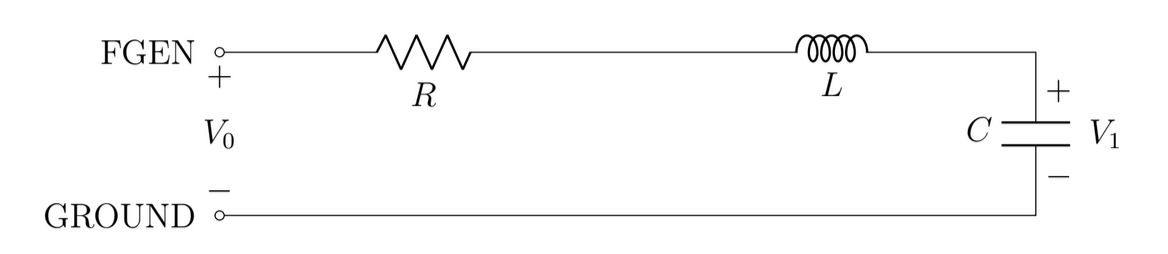
\includegraphics[scale=0.5]{figuras/circuito1}
\end{table}

\begin{center}
Figura 1: Circuito RLC com medição no capacitor
\end{center}

Usando o o gerador de funções do Elvis para gerar um onda senoidal com 4 Vpp, offset zero e frequência 10kHz e osciloscópio integrado ao Elvis para medir as tensões $V_0$ e $V_1$, é obtido o Gráfico 1.


\begin{table}[h]
\centering
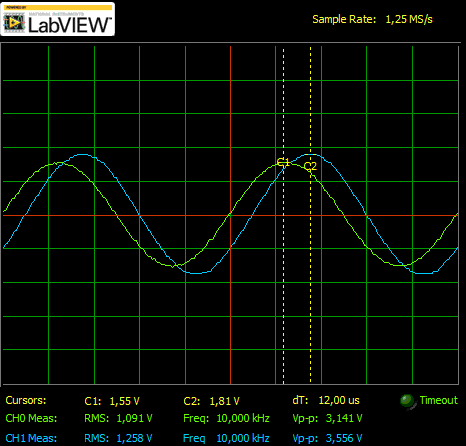
\includegraphics[scale=0.7]{graficos/circ1/rgadicoa1-2-10}
\end{table}

\begin{center}
Gráfico 1: Coleta das tensões $V_1$ e $V_0$ no capacitor a 10kHz
\end{center}

Com isso obtemos os valores das amplitudes $|V_0|$, $|V_1|$ e a sua diferença de fase obtida através do dt, multiplicando simplesmente o dt por $\omega\cdot2\pi$. Como $\omega = 10^4$, a diferença de fase é de $-43.20$\textdegree, as amplitudes são $|V_0|=1.55V$, $|V_1|=1.81V$. Além disso, usando os valores das amplitudes das tensões é calculado o ganho da amplitude em decibéis através da fórmula $20log_{10}\left(\frac{|V_1|}{|V_0|}\right) = 1.347$ e esses valores são todos adicionados à Tabela 2.

Para o cálculo dos valores teóricos, é usada a fórmula de divisor de tensão para identificar os valores de $V_0$ e $V_1$. Na frequência de 10kHz, a impedância total do circuito é de $97-j990$ e a do capacitor é de $-j1000$. Portanto,

\[V_0 = 2\cdot\frac{47-j990}{97-j990}=1.57\angle-19.19\text{\textdegree}V\]
\[V_1=2\cdot\frac{-j1000}{97-j990}=2.33\angle-45.20\text{\textdegree}V\]
\[20log_{10}\left(\frac{|V_1|}{|V_0|}\right)=3.434\]
\[\text{Diferença de fase: }-26.01\text{\textdegree}\]

Esses valores também são adicionados à Tabela 2.

Em seguida, o processo é repetido com as frequências de 12.5kHz, 15.5kHz, 19.3kHz, 24.1kHz e 30kHz. Como as contas são todas completamente análogas, elas serão omitidas, mas seus resultados constam na Tabela 2. Seguem a seguir o gráfico 2, Gráfico 3, Gráfico 4, Gráfico 5 e Gráfico 6 para as próximas frequências.


\begin{table}[h]
\centering
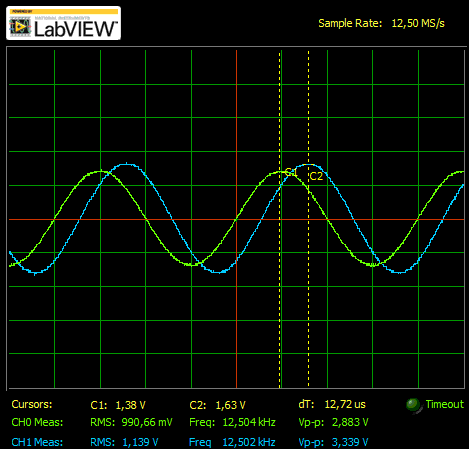
\includegraphics[scale=0.7]{graficos/circ1/rgadicoa1-2-12_5}
\end{table}

\begin{center}
Gráfico 2: Coleta das tensões $V_1$ e $V_0$ no capacitor a 12.5kHz
\end{center}

\newpage
\begin{table}[h]
\centering
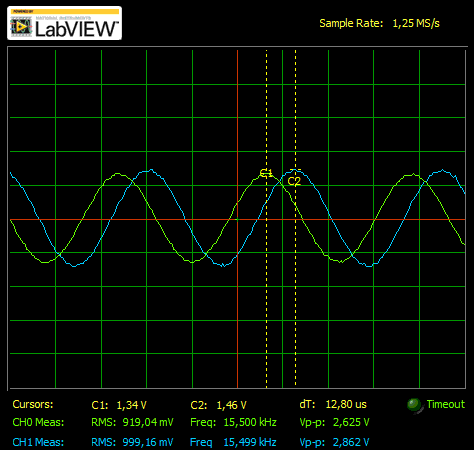
\includegraphics[scale=0.7]{graficos/circ1/rgadicoa1-2-15_5}
\end{table}

\begin{center}
Gráfico 3: Coleta das tensões $V_1$ e $V_0$ no capacitor a 15.5kHz
\end{center}


\begin{table}[h]
\centering
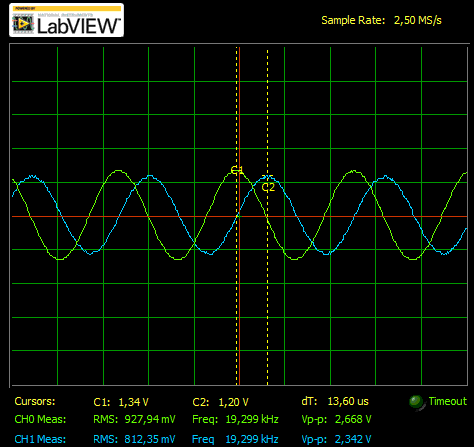
\includegraphics[scale=0.7]{graficos/circ1/rgadicoa1-2-19_3}
\end{table}

\begin{center}
Gráfico 4: Coleta das tensões $V_1$ e $V_0$ no capacitor a 19.3kHz
\end{center}

\newpage
\begin{table}[h]
\centering
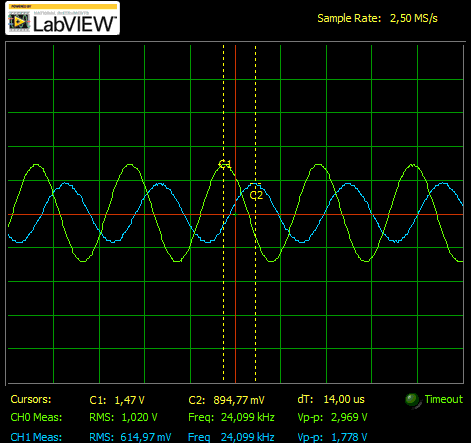
\includegraphics[scale=0.7]{graficos/circ1/rgadicoa1-2-24_1}
\end{table}

\begin{center}
Gráfico 5: Coleta das tensões $V_1$ e $V_0$ no capacitor a 24.1kHz
\end{center}


\begin{table}[h]
\centering
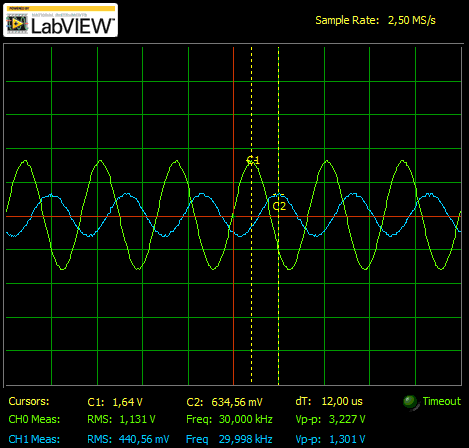
\includegraphics[scale=0.7]{graficos/circ1/rgadicoa1-2-30}
\end{table}

\begin{center}
Gráfico 6: Coleta das tensões $V_1$ e $V_0$ no capacitor a 30kHz
\end{center}

\newpage
\vspace{5pt}
\begin{table}[h]
\centering
\begin{tabular}{|c|c|c|c|c|}
\hline
\textbf{Frequência (kHz)} & \textbf{Grandeza} & \textbf{Valor nominal} & \textbf{Valor medido} & \textbf{Erro (\%) }\\\hline
10   & $|V_0|$ & 1.57V & 1.55V & 1.27 \\\hline
10   & $|V_1|$ & 2.33V & 1.81V & 22.31 \\\hline
10   & $20log_{10}(|V_1|/|V_0|)$ & 3.434 & 1.347 & 60.77 \\\hline
10   & Fase de $V_1$ em relação a $V_0$ & -26.01\textdegree & -43.20\textdegree & 66.09 \\\hline
12.5 & $|V_0|$ & 1.25V & 1.38V & 10.40 \\\hline
12.5 & $|V_1|$ & 2.35V & 1.63V & 30.64 \\\hline
12.5 & $20log_{10}(|V_1|/|V_0|)$ & 5.481 & 1.446 & 73.62 \\\hline
12.5 & Fase de $V_1$ em relação a $V_0$ & -43.93\textdegree & -57.24\textdegree & 30.30 \\\hline
15.5 & $|V_0|$ & 0.97V & 1.34V & 38.14 \\\hline
15.5 & $|V_1|$ & 2.11V & 1.46V & 30.81 \\\hline
15.5 & $20log_{10}(|V_1|/|V_0|)$ & 6.733 & 0.745 & 88.94 \\\hline
15.5 & Fase de $V_1$ em relação a $V_0$ & -83.58\textdegree & -71.45\textdegree & 14.51 \\\hline
19.3 & $|V_0|$ & 1.17V & 1.34V & 14.53 \\\hline
19.3 & $|V_1|$ & 1.58V & 1.20V & 24.05 \\\hline
19.3 & $20log_{10}(|V_1|/|V_0|)$ & 2.626 & -0.958 & 136.48 \\\hline
19.3 & Fase de $V_1$ em relação a $V_0$ & -129.54\textdegree & -94.48\textdegree & 27.06 \\\hline
24.1 & $|V_0|$ & 1.51V & 1.47V & 2.65 \\\hline
24.1 & $|V_1|$ & 1.02V & 0.89V & 12.75 \\\hline
24.1 & $20log_{10}(|V_1|/|V_0|)$ & -3.381 & -4.359 & 28.93 \\\hline
24.1 & Fase de $V_1$ em relação a $V_0$ & -151.17\textdegree & -121.47\textdegree & 19.65 \\\hline
30   & $|V_0|$ & 1.72V & 1.64V & 4.65 \\\hline
30   & $|V_1|$ & 0.64V & 0.63V & 1.56 \\\hline
30   & $20log_{10}(|V_1|/|V_0|)$ & -8.635 & -4.155 & 51.88 \\\hline
30   & Fase de $V_1$ em relação a $V_0$ & -160.86\textdegree & -129.49\textdegree & 19.51 \\\hline
\end{tabular}
\caption*{Tabela 2: Valores referentes ao circuito 1}
\end{table}


Agora que a Tabela 2 está completa, o circuito sofre uma alteração e sua configuração agora é de acordo com a Figura 2:

\begin{table}[h]
\centering
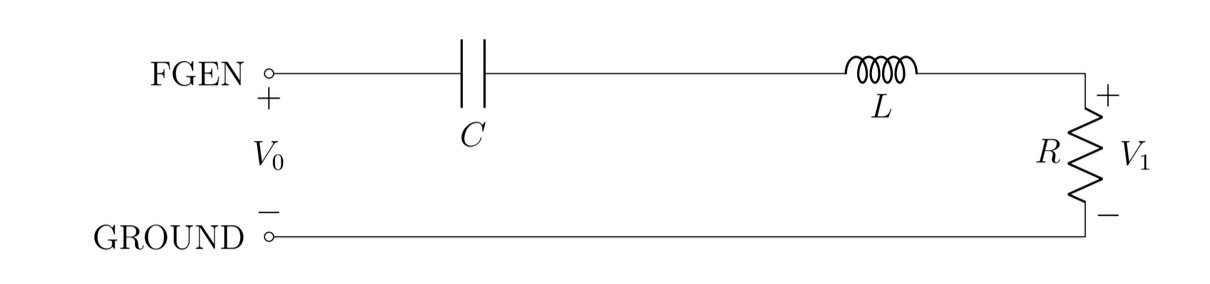
\includegraphics[scale=0.5]{figuras/circuito2}
\end{table}

\begin{center}
Figura 2: Circuito RLC com medição no resistor.
\end{center}

No entanto, todas as medições são exatamente análogas, mudando apenas que no divisor de tensão usa-se agora a resistência de 47$\Omega$ em vez da impedância do capacitor, portanto serão omitidas. Seguem os gráficos obtidos experimentalmente.

\newpage
\begin{table}[h]
\centering
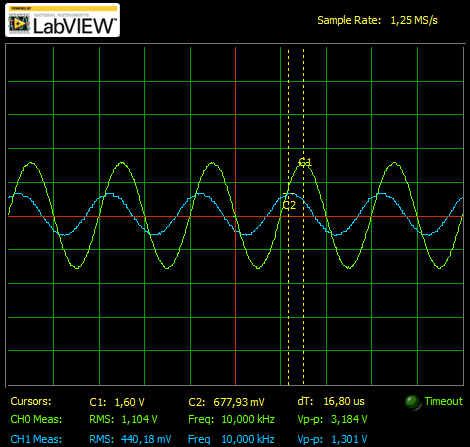
\includegraphics[scale=0.7]{graficos/circ2/rgadicoa2-2-10}
\end{table}

\begin{center}
Gráfico 7: Coleta das tensões $V_1$ e $V_0$ no resistor a 10kHz
\end{center}

\begin{table}[h]
\centering
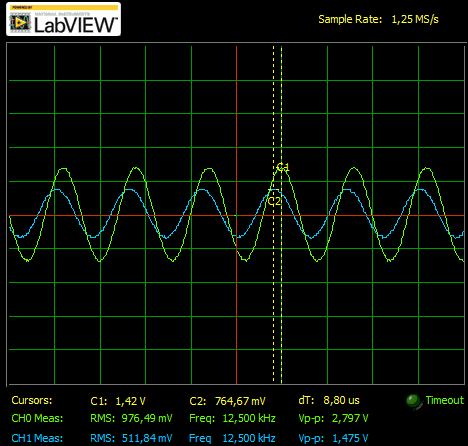
\includegraphics[scale=0.7]{graficos/circ2/rgadicoa2-2-12_5}
\end{table}

\begin{center}
Gráfico 8: Coleta das tensões $V_1$ e $V_0$ no resistor a 12.5kHz
\end{center}

\newpage
\begin{table}[h]
\centering
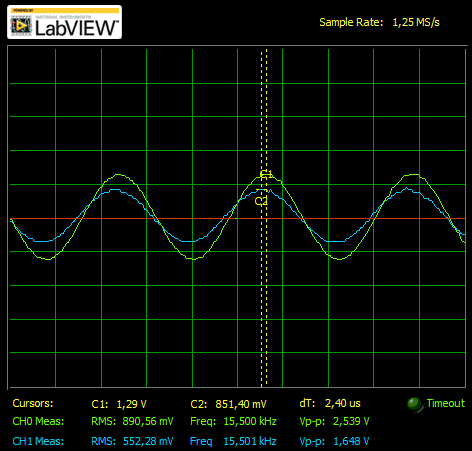
\includegraphics[scale=0.7]{graficos/circ2/rgadicoa2-2-15_5}
\end{table}

\begin{center}
Gráfico 9: Coleta das tensões $V_1$ e $V_0$ no resistor a 15.5kHz
\end{center}

\begin{table}[h]
\centering
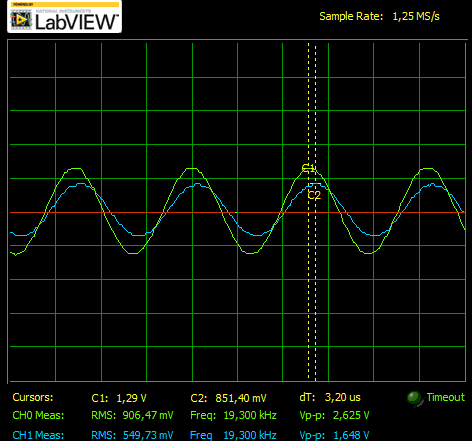
\includegraphics[scale=0.7]{graficos/circ2/rgadicoa2-2-19_3}
\end{table}

\begin{center}
Gráfico 10: Coleta das tensões $V_1$ e $V_0$ no resistor a 19.3kHz
\end{center}

\newpage
\begin{table}[h]
\centering
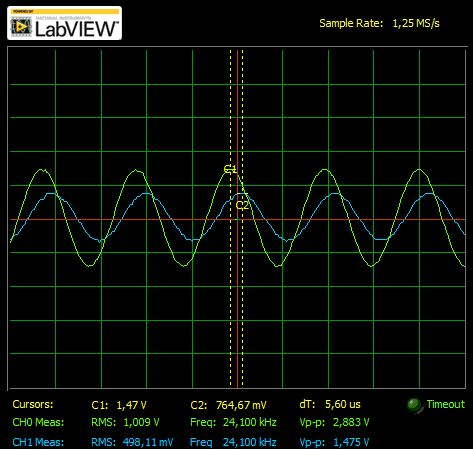
\includegraphics[scale=0.7]{graficos/circ2/rgadicoa2-2-24_1}
\end{table}

\begin{center}
Gráfico 11: Coleta das tensões $V_1$ e $V_0$ no resistor a 24.1kHz
\end{center}

\begin{table}[h]
\centering
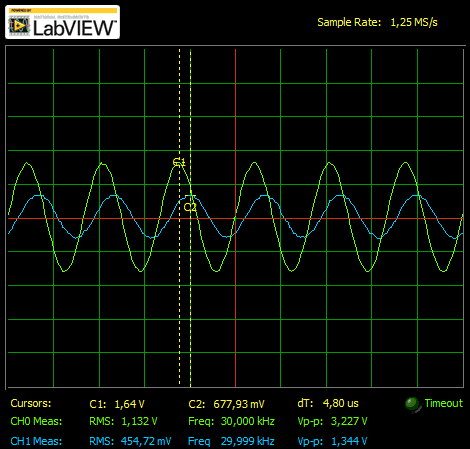
\includegraphics[scale=0.7]{graficos/circ2/rgadicoa2-2-30}
\end{table}

\begin{center}
Gráfico 12: Coleta das tensões $V_1$ e $V_0$ no resistor a 30kHz
\end{center}

Todos os valores para o segundo circuito estão na Tabela 3.

\newpage
\vspace{5pt}
\begin{table}[h]
\centering
\begin{tabular}{|c|c|c|c|}
\hline
\textbf{Grandeza} & \textbf{Valor nominal} & \textbf{Valor medido} & \textbf{Erro (\%) }\\\hline
$v_0$ & 1V & 1.006V & 0.6 \\\hline
$v_1$ & 3.2V & 2.315V & 27.66 \\\hline
$v_-$ & 1V & 1.007V & 0.7 \\\hline
$V^+$ & 10V & 9.994V & 0.6 \\\hline
$V^-$ & -10V & -10.005V & 0.5 \\\hline
$i_+$ & 0A & 0.195A & - \\\hline
$i_-$ & 0A & 4.158mA & - \\\hline
\end{tabular}
\caption*{Tabela 1: Valores dos componentes}
\end{table}

Assim como foi feito anteriormente, agora o circuito muda mais uma vez e fica de acordo com a Figura 3.

\begin{table}[h]
\centering
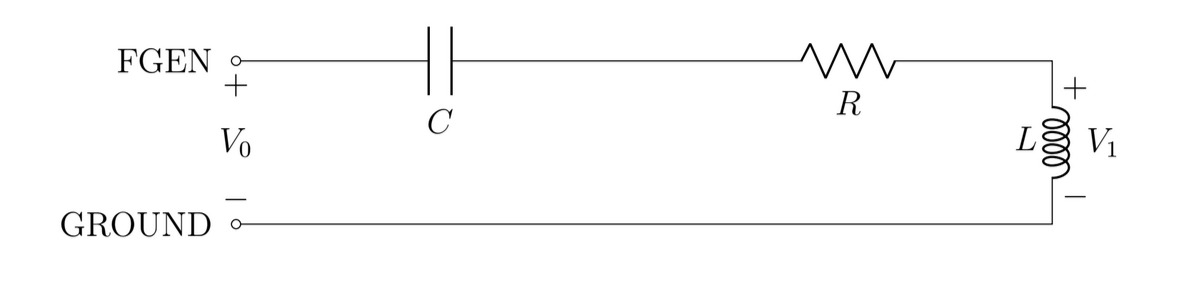
\includegraphics[scale=0.5]{figuras/circuito3}
\end{table}

\begin{center}
Figura 2: Circuito RLC com medição no indutor.
\end{center}

Novamente, os cálculos são completamente análogos, mudando apenas a fórmula do divisor de tensão para a tensão no indutor. Logo, os cálculos serão omitidos e seus resultados dispostos na Tabela 4, logo após os gráficos experimentais.

	\newpage
	\begin{table}[h]
	\centering
	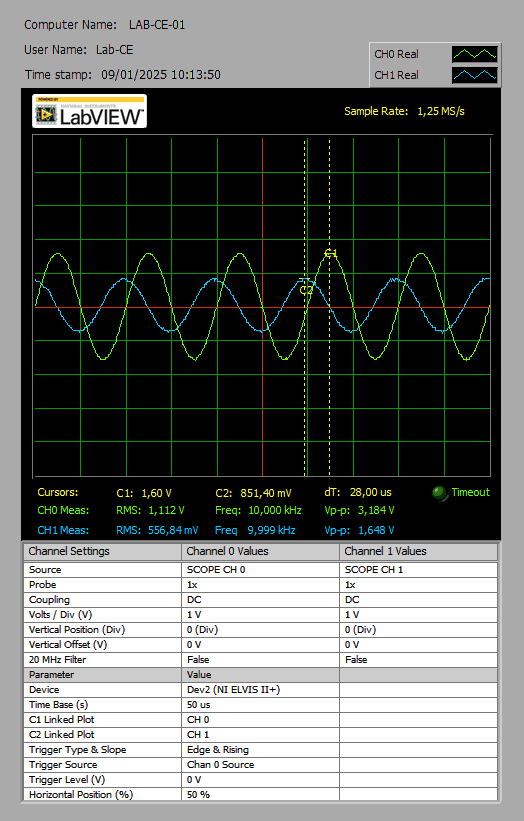
\includegraphics[scale=0.7]{graficos/circ3/rgadicoa3-2-10}
	\end{table}
	
	\begin{center}
	Gráfico 13: Coleta das tensões $V_1$ e $V_0$ no indutor a 10kHz
	\end{center}

	
	\begin{table}[h]
	\centering
	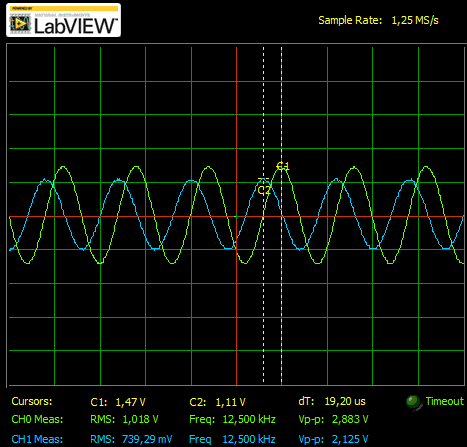
\includegraphics[scale=0.7]{graficos/circ3/rgadicoa3-2-12_5}
	\end{table}
	
	\begin{center}
	Gráfico 14: Coleta das tensões $V_1$ e $V_0$ no indutor a 12.5kHz
	\end{center}

	\newpage
	\begin{table}[h]
	\centering
	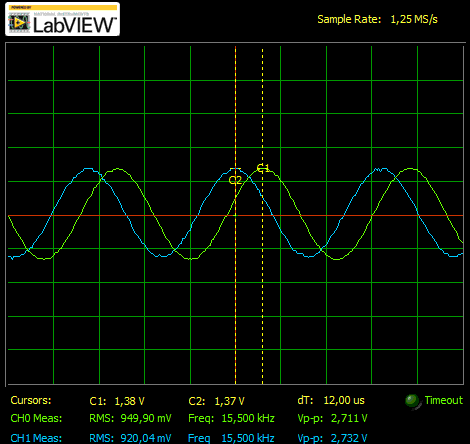
\includegraphics[scale=0.7]{graficos/circ3/rgadicoa3-2-15_5}
	\end{table}
	
	\begin{center}
	Gráfico 15: Coleta das tensões $V_1$ e $V_0$ no indutor a 15.5kHz
	\end{center}

	
	\begin{table}[h]
	\centering
	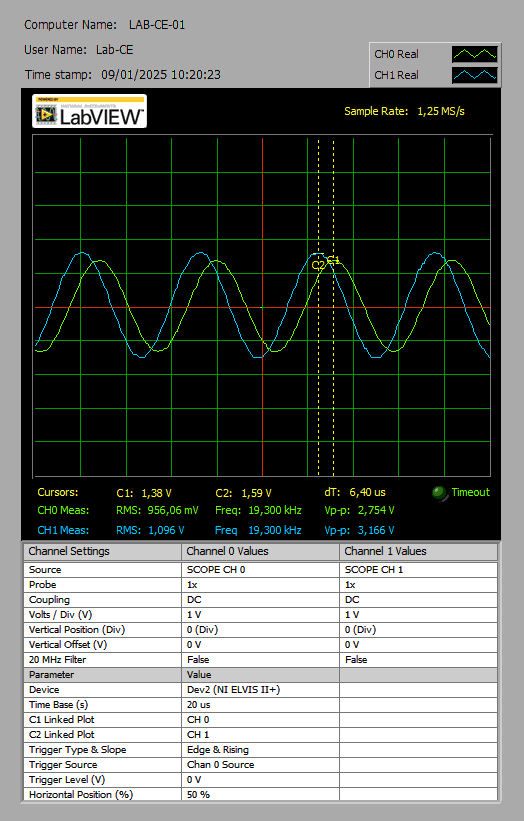
\includegraphics[scale=0.7]{graficos/circ3/rgadicoa3-2-19_3}
	\end{table}
	
	\begin{center}
	Gráfico 16: Coleta das tensões $V_1$ e $V_0$ no indutor a 19.3kHz
	\end{center}

	\newpage
	\begin{table}[h]
	\centering
	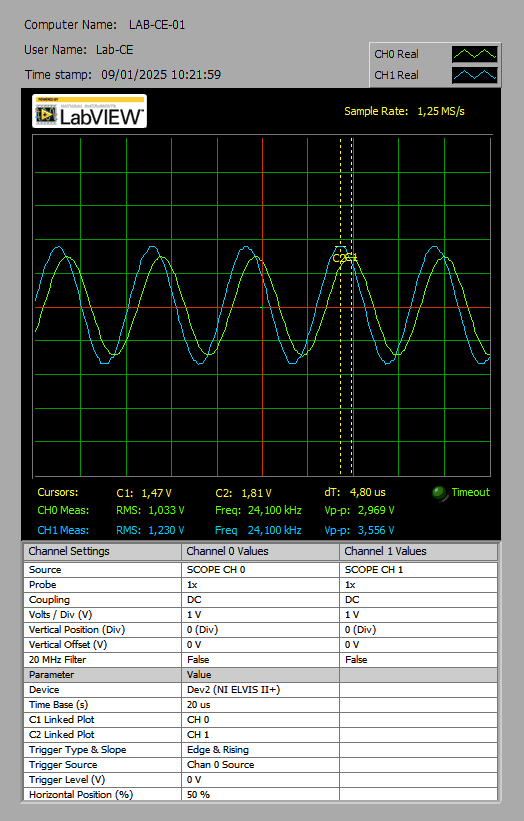
\includegraphics[scale=0.7]{graficos/circ3/rgadicoa3-2-24_1}
	\end{table}
	
	\begin{center}
	Gráfico 17: Coleta das tensões $V_1$ e $V_0$ no indutor a 24.1kHz
	\end{center}

	
	\begin{table}[h]
	\centering
	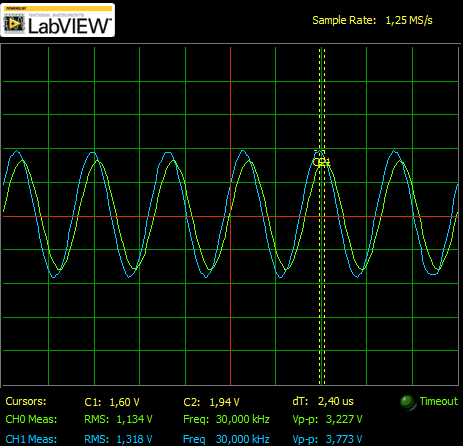
\includegraphics[scale=0.7]{graficos/circ3/rgadicoa3-2-30}
	\end{table}
	
	\begin{center}
	Gráfico 18: Coleta das tensões $V_1$ e $V_0$ no indutor a 30kHz
	\end{center}

Todos os valores para o terceiro circuito estão na Tabela 4.

\newpage
\vspace{5pt}
\begin{table}[h]
\centering
\begin{tabular}{|c|c|c|c|c|}
\hline
\textbf{Frequência (kHz)} & \textbf{Grandeza} & \textbf{Valor nominal} & \textbf{Valor medido} & \textbf{Erro (\%) }\\\hline
10   & $|V_0|$ &  & 1.60V &  \\\hline
10   & $|V_1|$ &  & 0.85V &  \\\hline
10   & $20log_{10}(|V_1|/|V_0|)$ &  & -5.494 &  \\\hline
10   & Fase de $V_1$ em relação a $V_0$ &  & -100.78\textdegree &  \\\hline
12.5 & $|V_0|$ &  & 1.47V &  \\\hline
12.5 & $|V_1|$ &  & 1.11V &  \\\hline
12.5 & $20log_{10}(|V_1|/|V_0|)$ &  & -2.439 &  \\\hline
12.5 & Fase de $V_1$ em relação a $V_0$ &  & -86.40\textdegree &  \\\hline
15.5 & $|V_0|$ &  & 1.38V &  \\\hline
15.5 & $|V_1|$ &  & 1.37V &  \\\hline
15.5 & $20log_{10}(|V_1|/|V_0|)$ &  & -0.063 &  \\\hline
15.5 & Fase de $V_1$ em relação a $V_0$ &  & -66.98\textdegree &  \\\hline
19.3 & $|V_0|$ &  & 1.38V &  \\\hline
19.3 & $|V_1|$ &  & 1.59V &  \\\hline
19.3 & $20log_{10}(|V_1|/|V_0|)$ &  & 1.230 &  \\\hline
19.3 & Fase de $V_1$ em relação a $V_0$ &  & -44.46\textdegree &  \\\hline
24.1 & $|V_0|$ &  & 1.47V &  \\\hline
24.1 & $|V_1|$ &  & 1.81V &  \\\hline
24.1 & $20log_{10}(|V_1|/|V_0|)$ &  & 1.807 &  \\\hline
24.1 & Fase de $V_1$ em relação a $V_0$ &  & -41.65\textdegree &  \\\hline
30   & $|V_0|$ &  & 1.60V &  \\\hline
30   & $|V_1|$ &  & 1.94V &  \\\hline
30   & $20log_{10}(|V_1|/|V_0|)$ &  & 1.673 &  \\\hline
30   & Fase de $V_1$ em relação a $V_0$ &  & -25.90\textdegree &  \\\hline
\end{tabular}
\caption*{Tabela 4: Valores referentes ao circuito 3}
\end{table}

\vspace{1cm}
Agora que temos todos os dados, passamos para a análise dos diagramas de Bode.
O diagrama de Bode é obtido através da análise em escala logarítmica da função de transferência do circuito no domínio fasorial. Para obter $H(j\omega)$, um dos métodos é através da técnica de divisores de tensão, isto é, utilizando a relação $V1 = V_0\cdot\left(\frac{Z_{carga}}{Z_{eq}}\right)$, obtém-se a razão V1/V0, equivalente à função de transferência. 

Para a resposta em amplitude, utiliza-se o módulo da função de transferência, sendo este convertido pelo fator $20log_{10}$, de modo que a análise do efeito da frequência passa a ser feita por década, oferecendo uma resposta em decibéis (dB), assim facilitando a análise para diferentes escalas de frequência.

Além disso, para o espectro de fase do circuito, calcula-se o ângulo da função de transferência, de modo que para obter a resposta, utilizamos a função arctan para definir o ângulo.

Para o circuito 1, onde a carga é o capacitor, tem-se a função de transferência $$H(j\omega)=\frac{-j10^7}{97\omega+j\frac{\omega^2}{1000} -j10^7}$$ de modo que sua resposta em amplitude resulta na figura 4 e sua resposta em frequência resulta na figura 5.

\newpage

\[|H(j\omega)|_{dB}=20log_{10}\left(\left|\frac{-j10^7}{97\omega+j\frac{\omega^2}{1000} -j10^7}\right|\right)\]

\textbf{$|H(j\omega)|$}
\begin{table}[h]
\centering
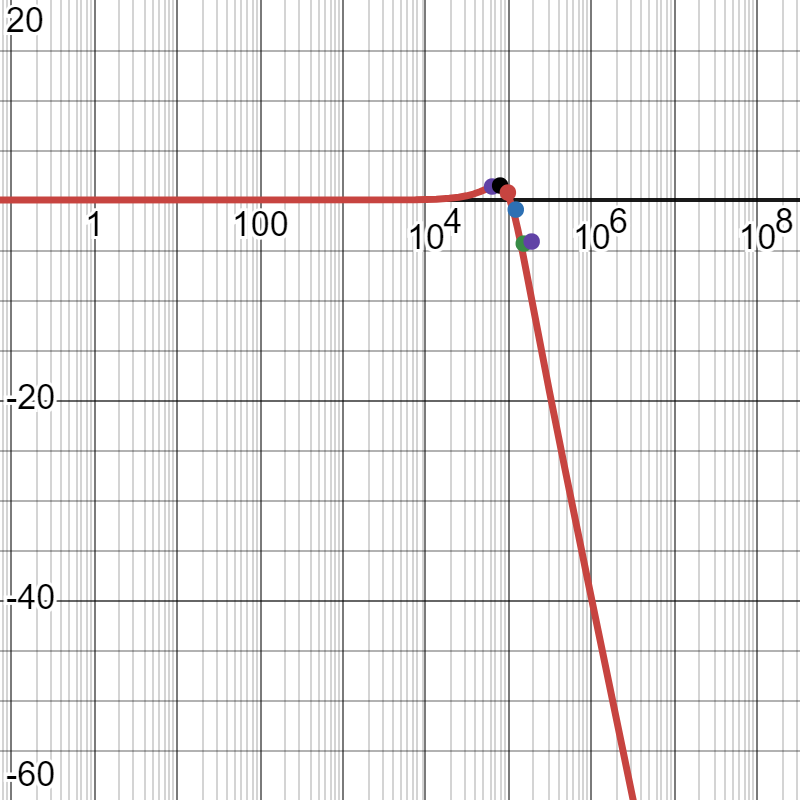
\includegraphics[scale=0.45]{figuras/bode-circ1}
\end{table}\vspace{-9.75cm}\marginpar{\textbf{$\omega$}}
\vspace{9.75cm}
\begin{table}[hb]
\centering
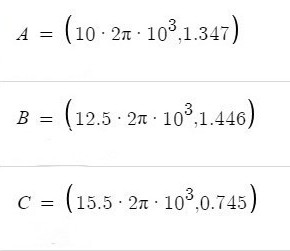
\includegraphics[scale=0.6]{figuras/pontosamplitude1-1}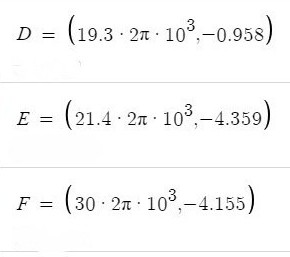
\includegraphics[scale=0.56]{figuras/pontosamplitude1}
\end{table}
\begin{center}
Figura 4: Diagrama de Bode da resposta em amplitude no circuito 1.
\end{center}

O traçado vermelho é o Diagrama de Bode usando os valores teóricos, enquanto os pontos são os experimentais e eles são definidos abaixo do diagrama.


\newpage
\[\angle H(j\omega) = \frac{\angle-j10^7}{\angle(97\omega+j\frac{\omega^2}{1000} -j10^7)}= -\frac{\pi}{2}-arctan\left(\frac{\frac{\omega}{1000}-\frac{10^7}{\omega}}{97}\right)\]
 
$\angle H(j\omega)$
\begin{table}[h]
\centering
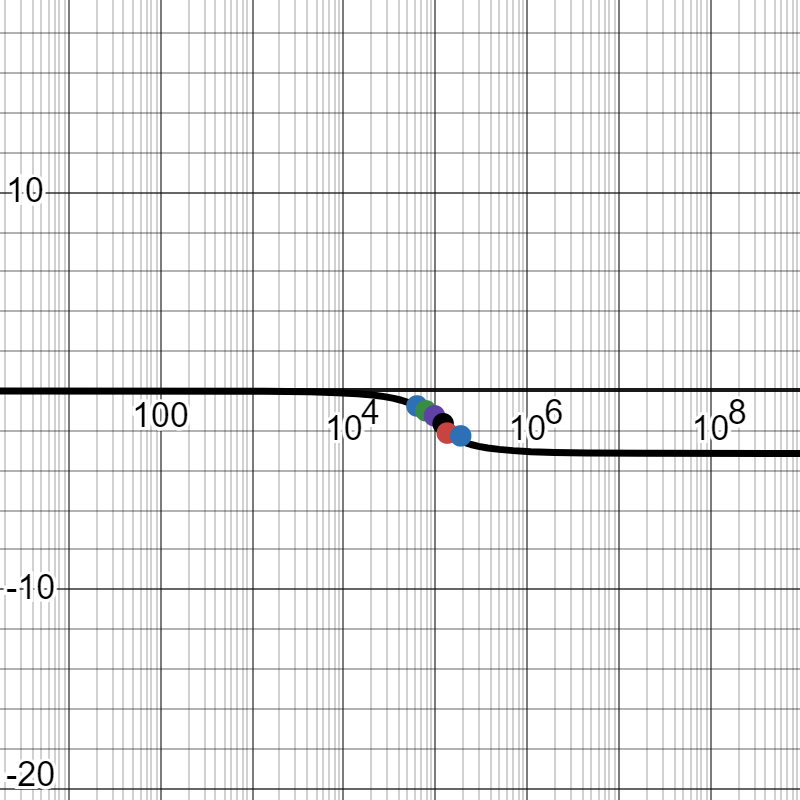
\includegraphics[scale=0.45]{figuras/circ1-fase}
\end{table}\vspace{-6.75cm}\marginpar{\textbf{$\omega$}}
\vspace{6.75cm}
\begin{table}[hb]
\centering
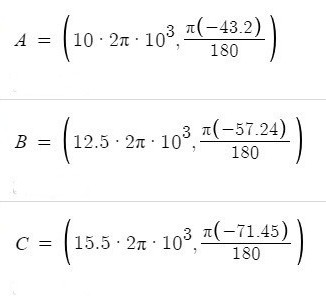
\includegraphics[scale=0.5]{figuras/pontosfase1-1}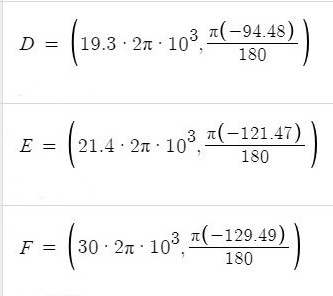
\includegraphics[scale=0.5]{figuras/pontosfase1}
\end{table}
\begin{center}
Figura 5: Diagrama de Bode da resposta em fase no circuito 1.
\end{center}

Para o circuito 2, onde a carga é o resistor, tem-se a função de transferência $$H(j\omega)=\frac{47\omega}{97\omega+j\frac{\omega^2}{1000}-j10^7}$$ de modo que sua resposta em amplitude resulta na Figura 6 e sua resposta em frequência resulta na Figura 7.

\[|H(j\omega)|_{dB} = 20log_{10}\left(\left|\frac{47\omega}{97\omega+j\frac{\omega^2}{1000}-j10^7}\right|\right)\]

$|H(j\omega)|$
\begin{table}[h]
\centering
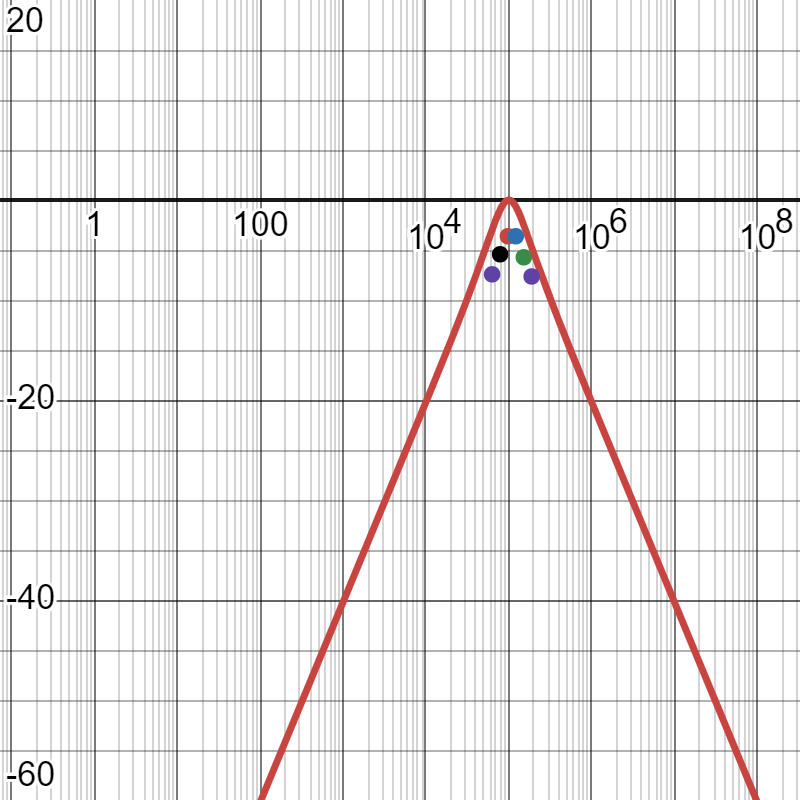
\includegraphics[scale=0.425]{figuras/bode-circ2}
\end{table}\vspace{-9.5cm}\marginpar{\textbf{$\omega$}}
\vspace{9.5cm}
\begin{table}[hb]
\centering
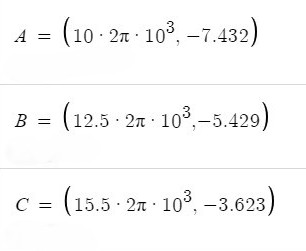
\includegraphics[scale=0.6]{figuras/pontosamplitude2-1}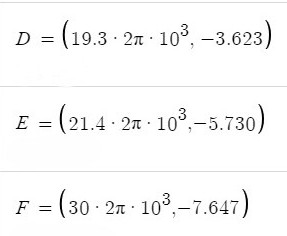
\includegraphics[scale=0.6]{figuras/pontosamplitude2}
\end{table}
\begin{center}
Figura 6: Diagrama de Bode da resposta em amplitude no circuito 2.
\end{center}


\newpage
\[\angle H(j\omega) = \angle 47\omega - \angle\left(97\omega+j\frac{\omega^2}{1000} -j10^7\right)=-arctan\left(\frac{\left(\frac{\omega}{1000}-\frac{10^7}{\omega}\right)}{97}\right)\]

\hspace{0.5cm}$\angle H(j\omega)$
\begin{table}[h]
\centering
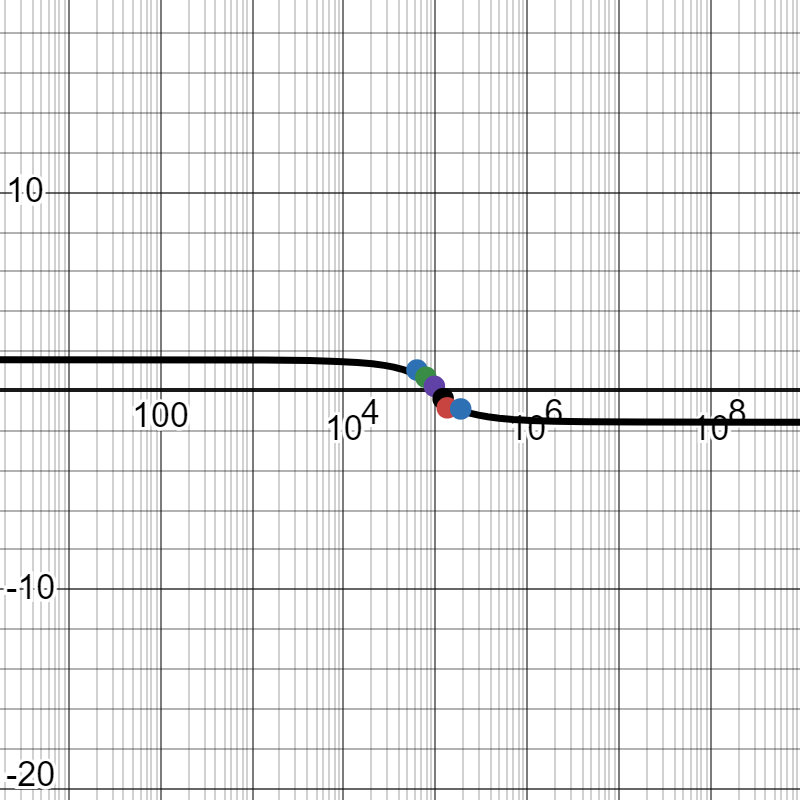
\includegraphics[scale=0.45]{figuras/circ2-fase}
\end{table}\vspace{-6.75cm}\marginpar{\textbf{$\omega$}}
\vspace{6.5cm}
\begin{table}[h]
\centering
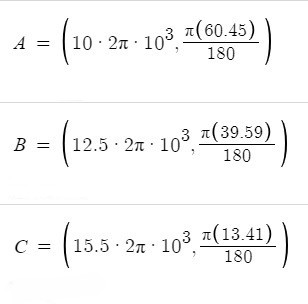
\includegraphics[scale=0.5]{figuras/pontosfase2-1}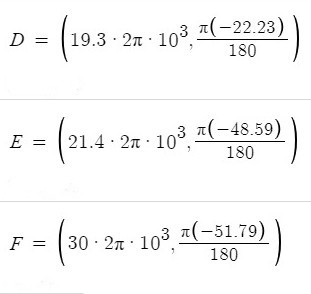
\includegraphics[scale=0.5]{figuras/pontosfase2}
\end{table}
\begin{center}
Figura 7: Diagrama de Bode da resposta em fase no circuito 2.
\end{center}

Para o circuito 3, onde a carga é o indutor, tem-se a função de transferência $$H(j\omega)=\frac{j\frac{\omega^2}{1000}}{97\omega+j\frac{\omega^2}{1000}-j10^7}$$ de modo que sua resposta em amplitude resulta na Figura 8 e sua resposta em frequência resulta na Figura 9.

\[|H(j\omega)|_{dB} = 20log_{10}\left(\left| \frac{j\frac{\omega^2}{1000}}{97\omega+j\frac{\omega^2}{1000}-j10^7} \right|\right)   \]


$|H(j\omega)|$
\begin{table}[h]
\centering
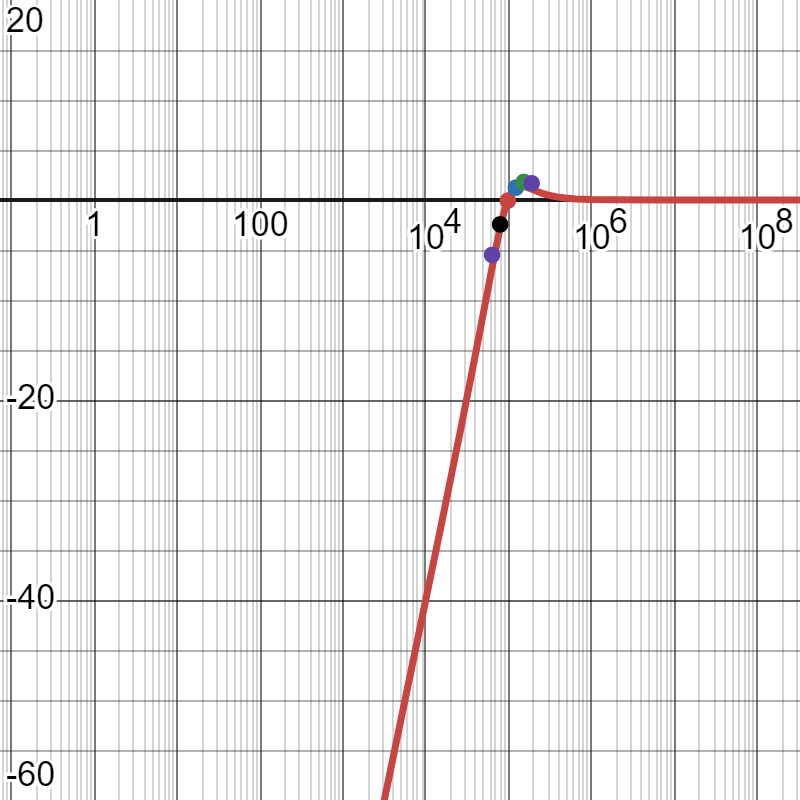
\includegraphics[scale=0.425]{figuras/bode-circ3}
\end{table}\vspace{-9.5cm}\marginpar{\textbf{$\omega$}}
\vspace{9cm}
\begin{table}[h]
\centering
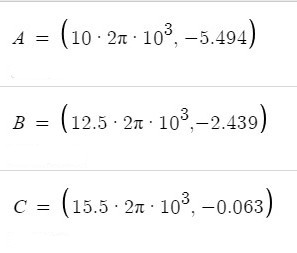
\includegraphics[scale=0.5]{figuras/pontosamplitude3-1}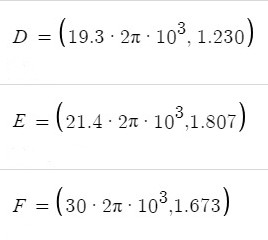
\includegraphics[scale=0.5]{figuras/pontosamplitude3}
\end{table}
\begin{center}
Figura 8: Diagrama de Bode da resposta em amplitude no circuito 3.
\end{center}


\newpage
\[\angle H(j\omega) = \angle\left(j\frac{\omega^2}{1000} \right)- \angle\left(97\omega+j\frac{\omega^2}{1000}-j10^7\right) = \frac{\pi}{2}-arctan\left(\frac{\left(\frac{\omega}{1000}-\frac{10^7}{\omega}\right)}{97}\right)\]

\hspace{0.5cm}$\angle H(j\omega)$
\begin{table}[h]
\centering
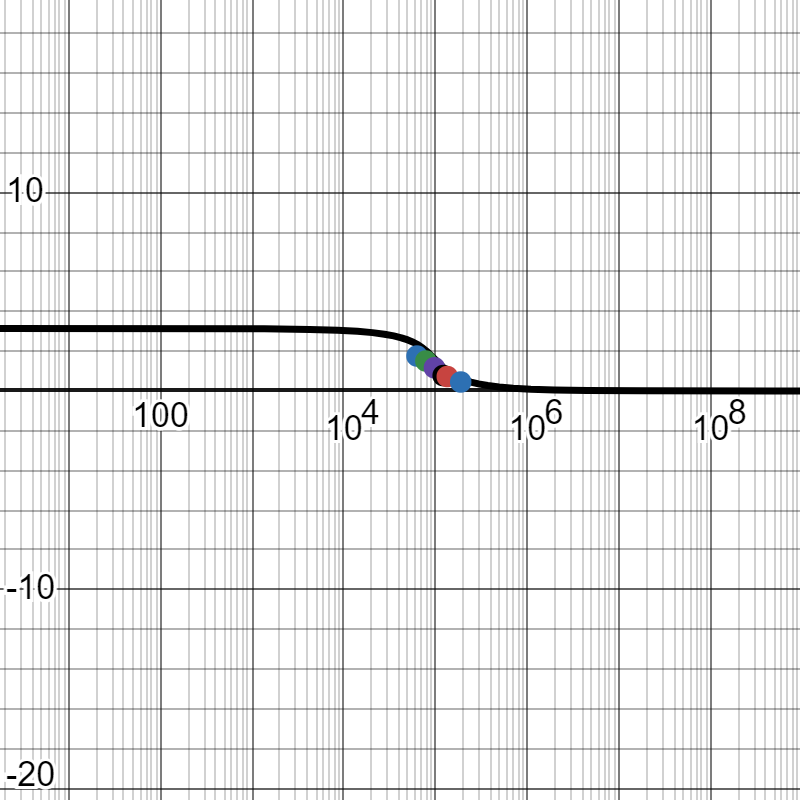
\includegraphics[scale=0.45]{figuras/circ3-fase}
\end{table}\vspace{-6.75cm}\marginpar{\textbf{$\omega$}}
\vspace{6.5cm}
\begin{table}[h]
\centering
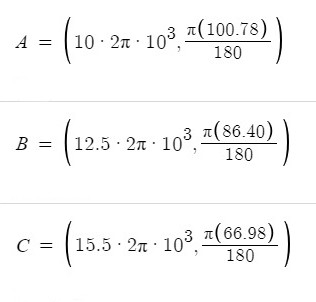
\includegraphics[scale=0.5]{figuras/pontosfase3-1}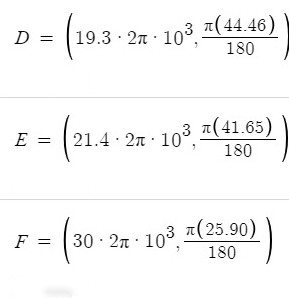
\includegraphics[scale=0.5]{figuras/pontosfase3}
\end{table}
\begin{center}
Figura 9: Diagrama de Bode da resposta em fase no circuito 3.
\end{center}


\section{Conclusão}
\parag O experimento permitiu a análise detalhada das respostas de amplitude e fase em função da frequência, evidenciando o impacto dos componentes resistivos, indutivos e capacitivos no comportamento do circuito. Foi possível determinar a frequência de ressonância, identificar regiões de ganho e atenuação e observar o comportamento de fase em diferentes faixas de frequência. Essas informações são fundamentais para o projeto e a aplicação de circuitos em sistemas que demandam controle de frequência, como filtros e amplificadores, consolidando a importância do Diagrama de Bode como ferramenta de análise no regime de sinais alternados.


\section{Bibliografia}

\begin{itemize}
\item HALLIDAY, D.; RESNICK, R.; WALKER, J. Fundamentos de Física. 10. ed. v. 3. Rio de Janeiro: LTC, 2016.
\end{itemize}


\end{document}